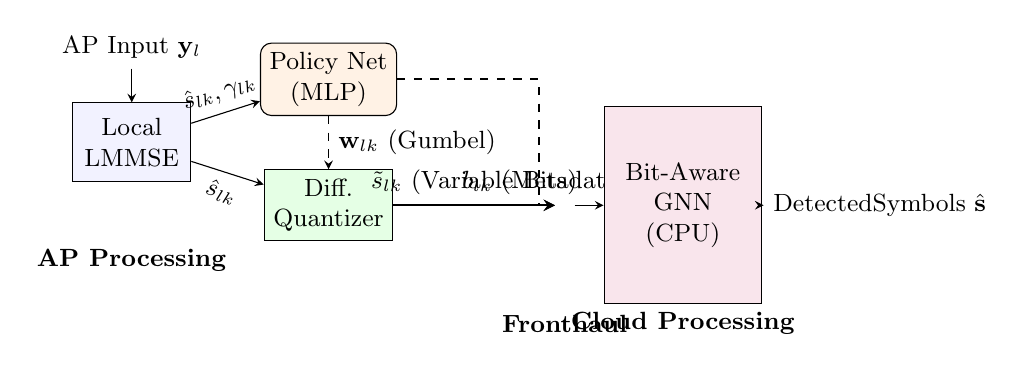
\begin{tikzpicture}[>=stealth, node distance=1.5cm, font=\small]

% Styles
\tikzstyle{block} = [draw, rectangle, minimum height=1cm, minimum width=1.5cm, align=center, fill=blue!5]
\tikzstyle{policy} = [draw, rectangle, minimum height=0.8cm, minimum width=1.2cm, align=center, fill=orange!10, rounded corners]
\tikzstyle{quant} = [draw, rectangle, minimum height=0.8cm, minimum width=1.2cm, align=center, fill=green!10]
\tikzstyle{gnn} = [draw, rectangle, minimum height=2.5cm, minimum width=2cm, align=center, fill=purple!10]

% Nodes - AP Side
\node[block] (lmmse) {Local\\LMMSE}; 
\node[above of=lmmse, node distance=1.2cm] (input) {AP Input $\mathbf{y}_l$}; 
\node[policy, right of=lmmse, node distance=2.5cm, yshift=0.8cm] (policy) {Policy Net\\(MLP)};
\node[quant, right of=lmmse, node distance=2.5cm, yshift=-0.8cm] (lsq) {Diff.\\Quantizer}; 

% Connections AP
\draw[->] (input) -- (lmmse);
\draw[->] (lmmse) -- node[above, sloped] {$\hat{s}_{lk}, \gamma_{lk}$} (policy);
\draw[->] (lmmse) -- node[below, sloped] {$\hat{s}_{lk}$} (lsq);
\draw[->, dashed] (policy) -- node[right] {$\mathbf{w}_{lk}$ (Gumbel)} (lsq);

% Fronthaul
\node[right of=lsq, node distance=3cm] (mid) {};
\draw[->, thick] (lsq) -- node[above] {$\tilde{s}_{lk}$ (Variable Bits)} (mid);
\draw[->, thick, dashed] (policy.east) -- ++(1.8,0) |- node[above, pos=0.7] {$b_{lk}$ (Metadata)} (mid);

% CPU Side
\node[gnn, right of=mid, node distance=1.5cm] (cpu) {Bit-Aware\\GNN\\(CPU)};
\node[right of=cpu, node distance=2.5cm] (output) {Detected\\Symbols $\hat{\mathbf{s}}$};

\draw[->] (mid) -- (cpu);
\draw[->] (cpu) -- (output);

% Labels
\node[below of=lmmse, node distance=1.5cm] {\textbf{AP Processing}};
\node[below of=mid, node distance=1.5cm] {\textbf{Fronthaul}};
\node[below of=cpu, node distance=1.5cm] {\textbf{Cloud Processing}};

\end{tikzpicture}